%%%%%%%%%%%%%%%%%%%%%%%%%%%%%%%%%%%%%%%%%%%%%%%%%%%%%%
%%%%%%%%%%%%%%%%%%%%%%%%TO DO %%%%%%%%%%%%%%%%%%%%%%%%
%%%%%%%%%%Colocar sobre projeto de estruturas aqui (colocar imagem esquemática, similar ao que foi feito na introdução), falar do ESMFold, AlphaFold...Falar sobre o DeNovo
%%%%%%%%%
%%%%%%%%%%%%%%%%%%%%%%%%%%%%%%%%%%%%%%%%%%%%%%%%%%%%%%


\chapter{Fundamentação teórica}
{\color{red} Em andamento}

Neste capítulo vamos apresentar alguns fundamentos teóricos utilizados neste trabalho acerca de proteínas e aprendizado por reforço profundo. 


\section{Proteina}
%O que é (sequencia de aminoácidos)
Uma proteína é uma macromolécula biológica composta por cadeias de aminoácidos. Constituem a maior parte da massa seca de uma célula, podendo desempenhar funções enzimáticas, estruturais, imonológicas, de transporte, entre outras \cite{Bio}. 

Existem milhares de proteínas diferentes em uma célula, onde cada uma é composta por uma sequência distinta dos 20 tipos de aminoácidos encontrados na natureza, unidos através de ligações peptídicas. Por conta disto, as proteínas são também conhecidas como polipeptídeos \cite{Bio}. 

A cadeia polipeptídica é composta por três componentes: a cadeia principal, as cadeias laterais e as ligações peptídicas. A cadeia principal é também referida como o esqueleto da proteína e é definida como uma série repetitiva e encadeada de átomos de carbono, nitrogénio e oxigénio. Anexadas a cadeia principal, encontram-se as cadeias laterais. Estas não estão envolvidas nas ligações peptídicas e são responsáveis por caracterizar as principais propriedades da proteína \cite{Bio}. 


\begin{figure}[H]
     \centering
     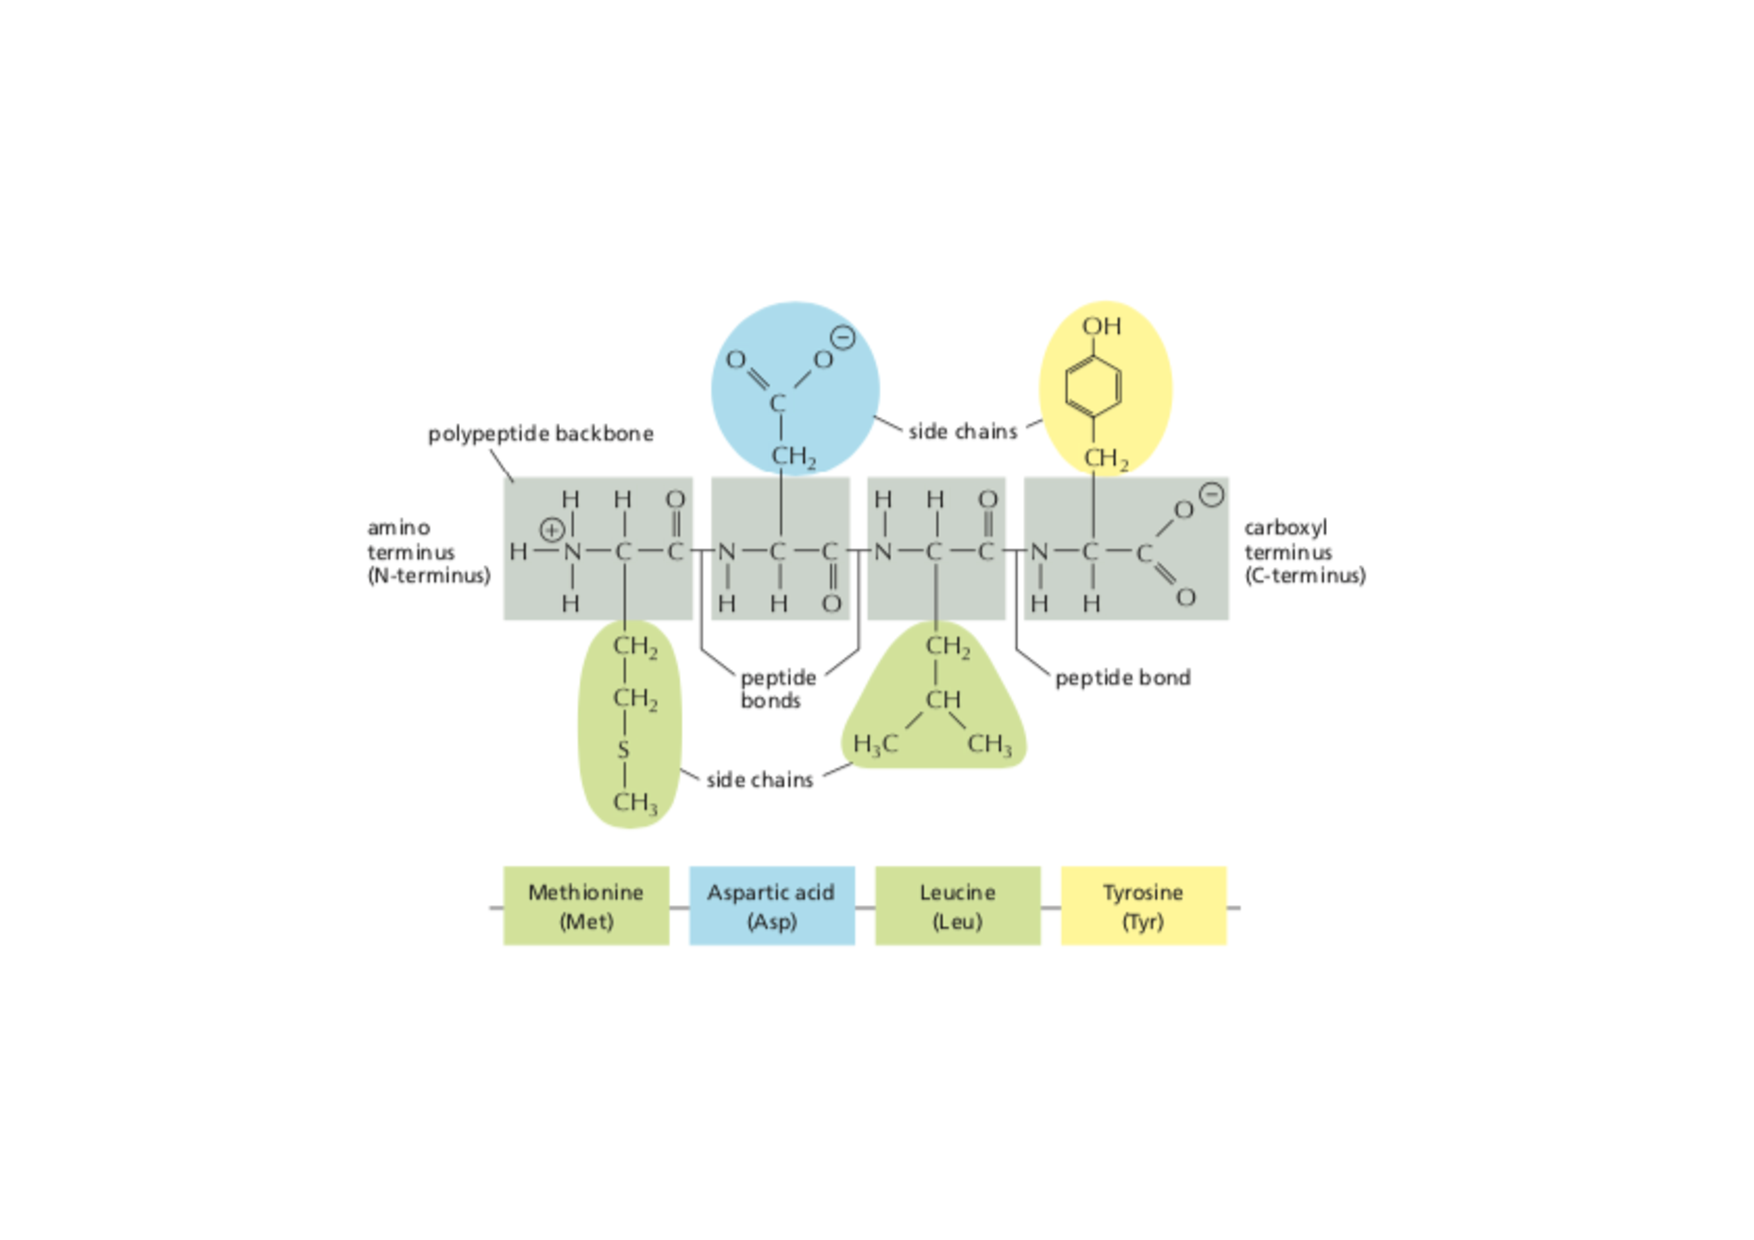
\includegraphics[width=0.6\textwidth]{figuras/ProteinBackbone.pdf}
     \caption{Componentes de uma proteína \cite{Bio}}
     %\label{Label de referência para a imagem}
\end{figure}


\begin{figure}[H]
     \centering
     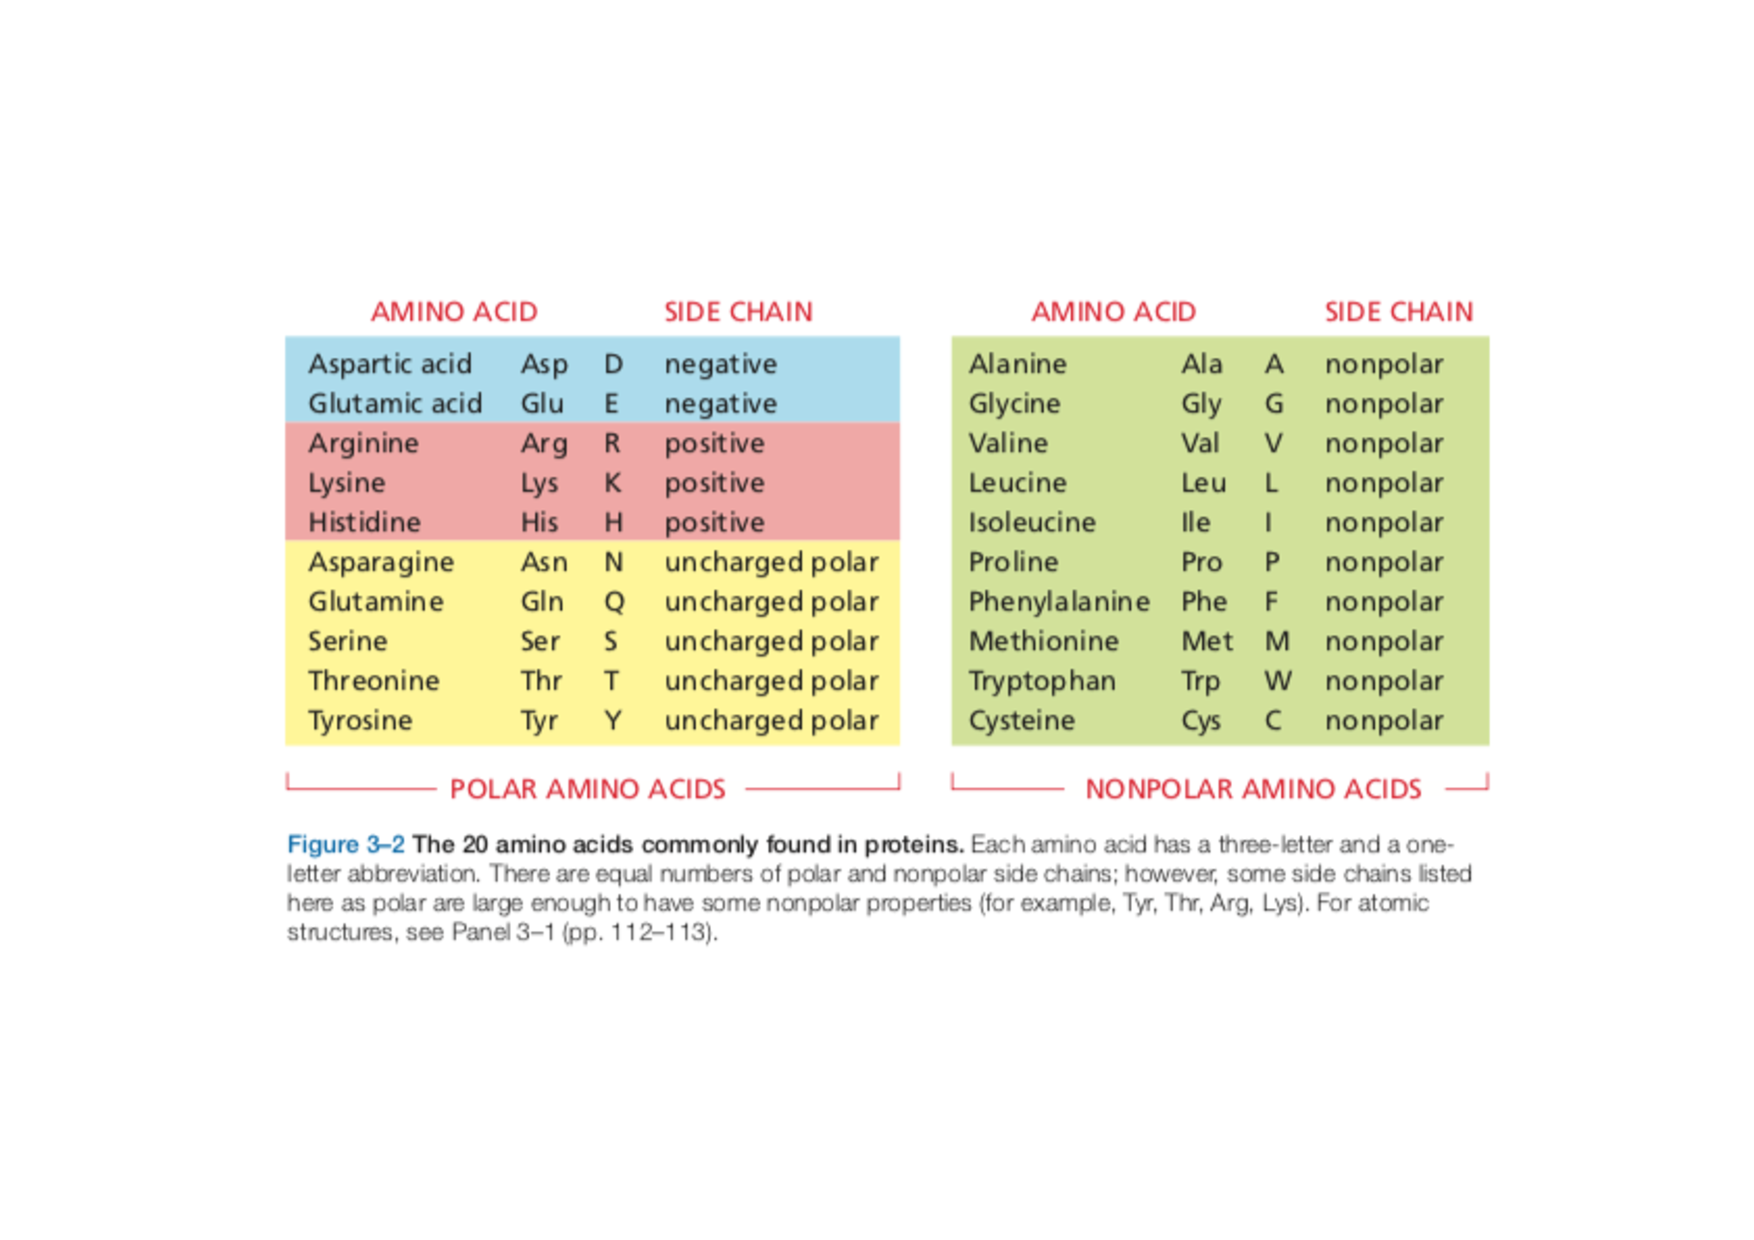
\includegraphics[width=0.6\textwidth]{figuras/20Aminoacidos.pdf}
     \caption{Os 20 aminoácidos \cite{Bio}}
     %\label{Label de referência para a imagem}
\end{figure}


\subsection{Estrutura proteíca}

A função de uma proteína está intimamente relacionada à sua estrutura tridimensional, que é formada principalmente a partir das interações entre as cadeias laterais e móleculas encontradas no meio físico ao qual a proteína está inserida. Devido a essas interações, a maioria das proteínas assume uma estrutura tridimensional única, que é determinada pela ordem dos aminoácidos na sequência. A conformação final tende a ser aquela que possui a menor energia livre \cite{Bio}.

\cite{Bio} explica que a polaridade das cadeias laterais desempenham um papel importante na predição estrutural da proteína. As cadeias não polares (hidrofóbicas) tendem a se agrupar no interior da molécula, evitando contato com a água. Já as polares tendem a se dispor perto da superfície da molécula, onde podem formar ligações de hidrogênio com a água e outras moléculas polares. 

\begin{figure}[H]
     \centering
     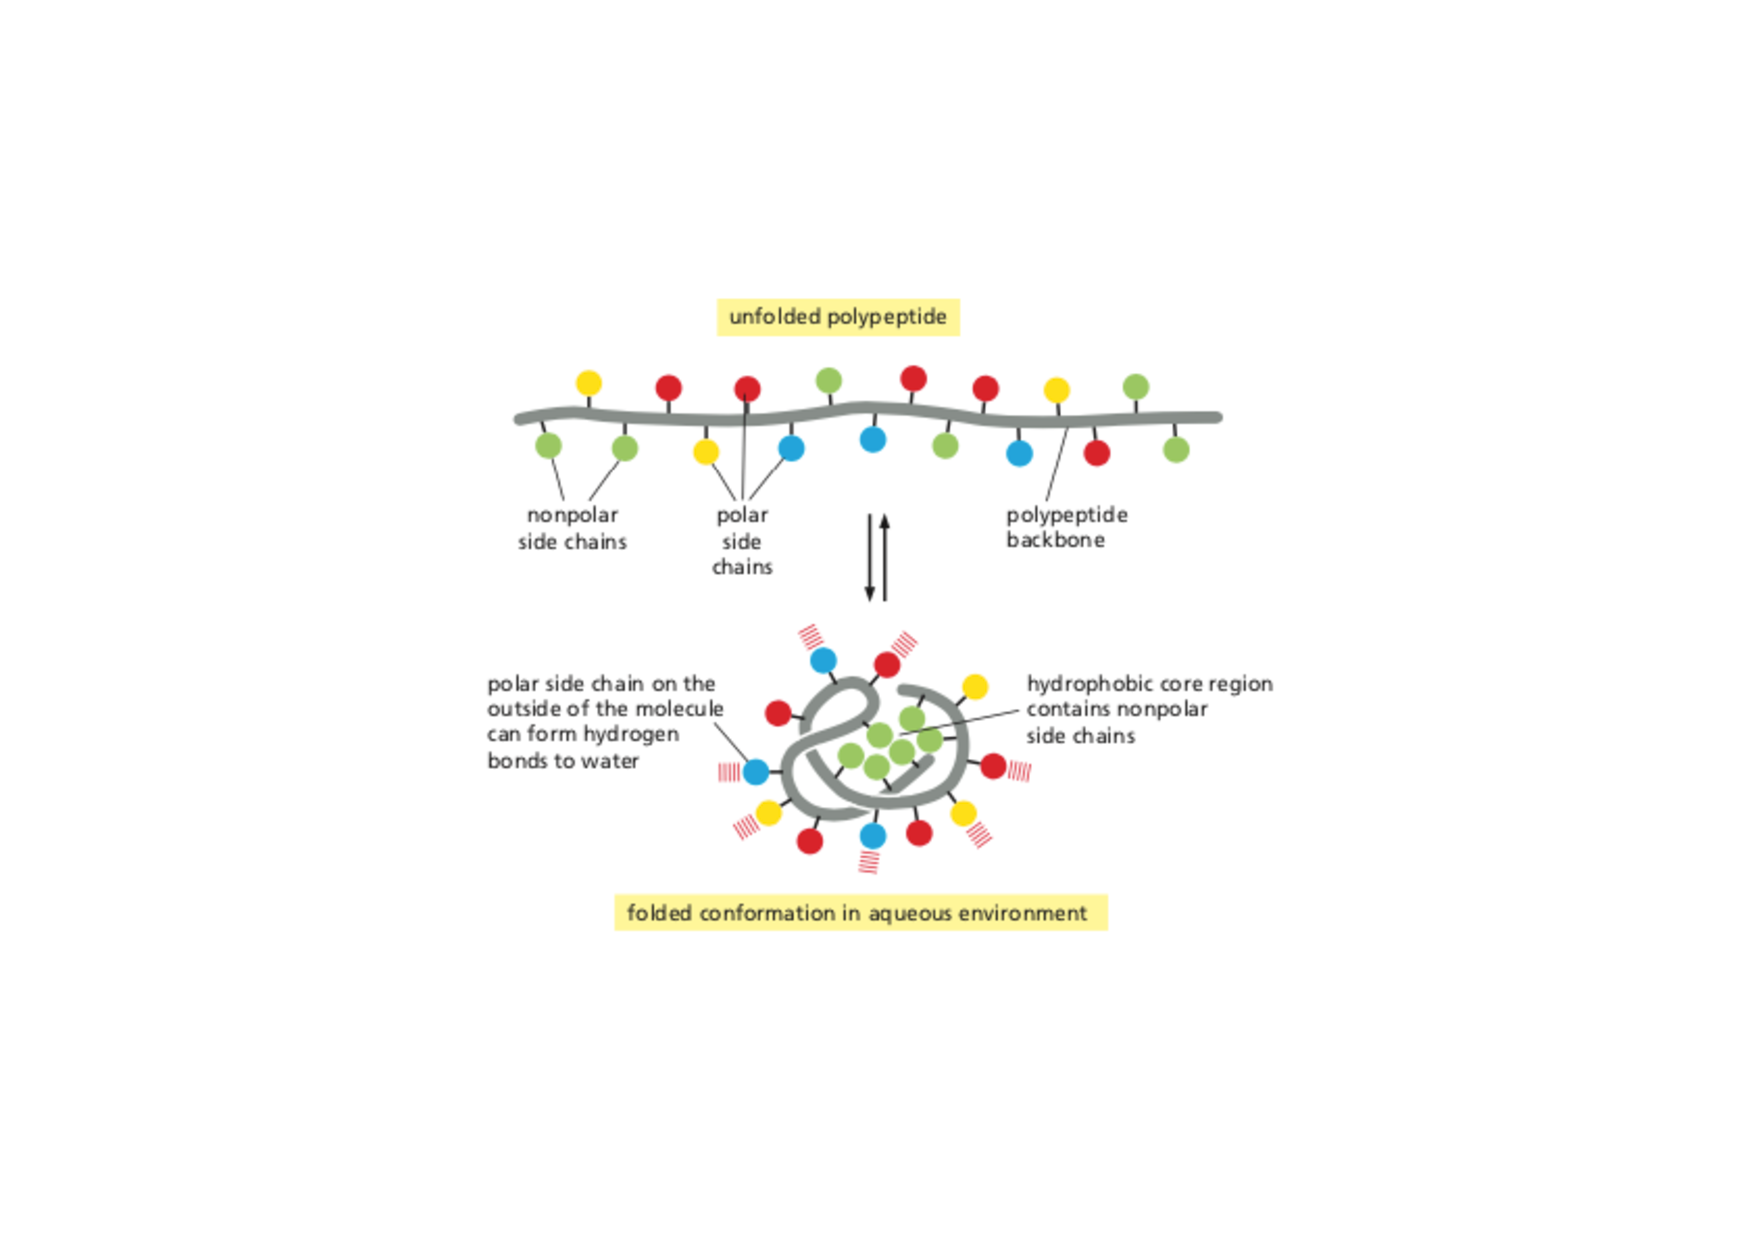
\includegraphics[width=0.6\textwidth]{figuras/ConformacaoProteica.pdf}
     \caption{Exemplo de conformação protéica \cite{Bio}}
     %\label{Label de referência para a imagem}
\end{figure}

\subsection{Resposta Imunológica}
{\color{red} TO DO}

\subsection{Afinidade de ligação}
{\color{red} TO DO}

\subsection{Estrutura alvo - Fator IX}
{\color{red} TO DO}
%Explicar o tamanho da sequencia, as especificidades, a resposta imunologica, a estabilidade
%citar Blood coagulation factor IX: structural insights impacting hemophilia B therapy
%https://ashpublications.org/blood/article-abstract/doi/10.1182/blood.2023023276/517006/Blood-coagulation-factor-IX-structural-insights?redirectedFrom=fulltext

\subsection{Mutação}
Uma mutação no contexto de proteínas refere-se a uma modificação na sequência de aminoácidos. Por menor que seja esta modificação, a mutação pode acarretar em uma alteração na estrutura tridimensional da proteína, uma vez que a ordem que os aminoácidos estão dispostos na sequência influencia diretamente na conformação da estrutura. Neste trabalho, vamos assumir que uma mutação consiste na substituição de apenas um aminoácido por outro na sequência. 

\subsection{Conservation Score}
O \textit{Conservation Score} (CS) é uma métrica que estima a importância ou contribuição individual de cada aminoácido da sequência na caracterização da função da proteína. Aminoácidos cruciais na estrutura da proteína tendem a ser conservados, visto que alterações neles podem impactar significativamente a função proteíca. 
O score é obtido levando-se em conta a frequência com que certas combinações de aminoácidos ocorrem em proteínas homólogas ao longo da evolução das espécies \cite{Eddy}. 
Para este trabalho, utilizamos o CS calculado pelo servidor ConsurfDB \cite{ConsurfDB}, tendo a estrutura do fator IX de coagulação como entrada. 
{\color{red} colocar uma imagem pra explicar}


\subsection{Similariedade entre aminoácidos}
Para mensurar o nível de similariedade entre os aminoácidos, utilizamos uma métrica de distância com base no trabalho \cite{aminodist}.
Nesse estudo, uma representação vetorial de 544 dimensões foi criada para cada aminoácido, incorporando informações sobre suas propriedades.
Essa representação foi desenvolvida com o auxílio do pacote seqinR \cite{seqinR}. 
Posteriormente, \cite{aminodist} aplicou uma redução de dimensionalidade com Principal Component Analysis (PCA), 
obtendo uma nova representação com 19 dimensões, retendo 99\% da informação original. 
Por fim, \cite{aminodist} apresenta a matriz de distâncias que iremos utilizar neste trabalho,
que é o resultado da distancia euclidiana entre cada par de vetores de 19 dimensões. 

\begin{figure}[H]
    \centering
    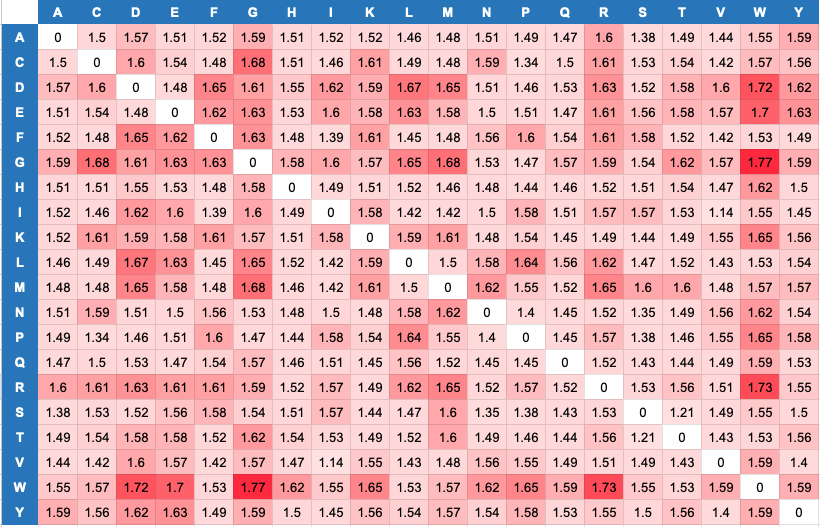
\includegraphics[width=.8\textwidth]{figuras/matrix_amino_dist.png}
    \caption{Distâncias entre pares de aminoácidos \cite{aminodist}}
    \label{fig:matrixaminodist}
  \end{figure}


\subsection{Similariedade entre estruturas}
\label{subsection:tmscore}
A métrica utilizada neste trabalho para mensurar a similariedade entre estruturas é o \textit{Template Matching Score} - \textit{TMScore}. 
Baseada principalmente em distâncias entre aminoácidos, o \textit{TMScore} é uma métrica que varia de 0 a 1,
sendo que quanto mais próximo de 1, maior será a similaridade entre as estruturas. 
Um TM-Score igual a 1 indica uma sobreposição perfeita e uma correspondência estrutural quase idêntica entre as proteínas, 
enquanto valores menores sugerem uma maior divergência estrutural entre elas. 
O cálculo desta medida foi feito a partir da plataforma desenvolvida por \cite{USalign}.
{\color{red} comparar com RMSD }


\section{Aprendizado por reforço profundo}
Nesta seção vamos introduzir os conceitos envolvidos no aprendizado por reforço profundo, que formam a base teórica da técnica que iremos utilizar: Proximal Policy Optimization (PPO). 
Para tal, será fornecido um contexto sobre Processo de Decisão de Markov (MDP), Redes Neurais (NN) e o método Ator-Crítico (AC). 


\subsection{Processo de Decisão de Markov}
O Processo de Decisão de Markov (MDP) é utilizado para modelar processos de forma probabilística. Ele é chamado de markoviano pois a distribuição de probabilidade de um estado depende apenas do estado anterior e da ação selecionada. Uma ação dá origem a um novo estado ao passo que promove alterações no estado atual. Um Agente seleciona cada ação com base em uma política ($\pi$) que mapeia estados a ações. Em um MDP, o processo evolui em etapas, ou \textit{steps}, à medida que o agente toma ações. A sequência de estados, desde o inicial até o final, é chamada de episódio. A qualidade de cada ação é avaliada com base no quão benéfico é o estado alcançado.
De acordo com \cite{MDP}, o MDP pode ser definido como uma tupla 
<S,A,T,R> onde:

\begin{itemize}
   \item S é o conjunto de possíveis estados;
   \item A é o conjunto de ações que interferem no processo;
   \item T :S×A×S$\rightarrow$[0,1] é uma função que quantifica a probabilidade de mudança do estado s $\in$ S para o estado $s'$ $\in$ S, dado a ação a $\in$ A selecionada. É representado por T ($s'$ |s, a);
   \item r : S × A$\rightarrow$r é uma função que mede a recompensa por selecionar a ação a $\in$ A quando o processo está no estado s $\in$ S.
 \end{itemize}

De modo a encontrar um bom $\pi$, é necessário definir uma maneira de comparar diferentes políticas. Uma técnica comum é comparar a esperança da recompensa acumulada descontada, ou Valor de Retorno (R), que cada política produziu em um mesmo episódio.

\begin{equation}
    R = E\begin{bmatrix} \sum_{k=1}^{z} \gamma ^{k-1} r_k \end{bmatrix}
\end{equation}

\noindent
Sendo z o tamanho do episódio, k o índice do \textit{step} e o $r_k$ a recompensa obtida em k. A constante $\gamma$ é um valor entre 0 e 1, chamado de fator de desconto. Ele é responsável por atribuir um peso maior a recompensas obtidas no início do episódio. 

Além disso, existem outras duas métricas importantes para se avaliar a qualidade de uma política: a Função de Valor (V) e a função de Valor da Ação (Q). A primeira estima a vantagem de estar em um estado s, calculando a esperança de R dado o estado inicial s0 = s. 

\begin{equation}
    V_\pi(s) = E[R|s_0 = s]
\end{equation}

A segunda estima a vantagem de selecionar a ação $a$ estando no estado $s$. Em outras palavras, é definida como a esperança de R dado o estado inicial e a ação inicial:

\begin{equation}
    Q_\pi(s,a) = E[R|s_0 = s, a_0 = a]
\end{equation}


Neste trabalho vamos modelar tanto a política $\pi$ quanto a Função de Valor V utilizando redes neurais profundas. 

\subsection{Redes Neurais}
Inspirado no sistema neural humano, uma rede neural artificial consiste em um conjunto de nós, chamados de neurônios, interconectados por arestas \cite{Bishop}. 
Em geral, é organizada em camadas, que incluem três tipos: a camada de entrada, a camada oculta e a camada de saída, conforme ilustrado na figura \ref{arqNN}.

\begin{figure}[H]
     \centering
     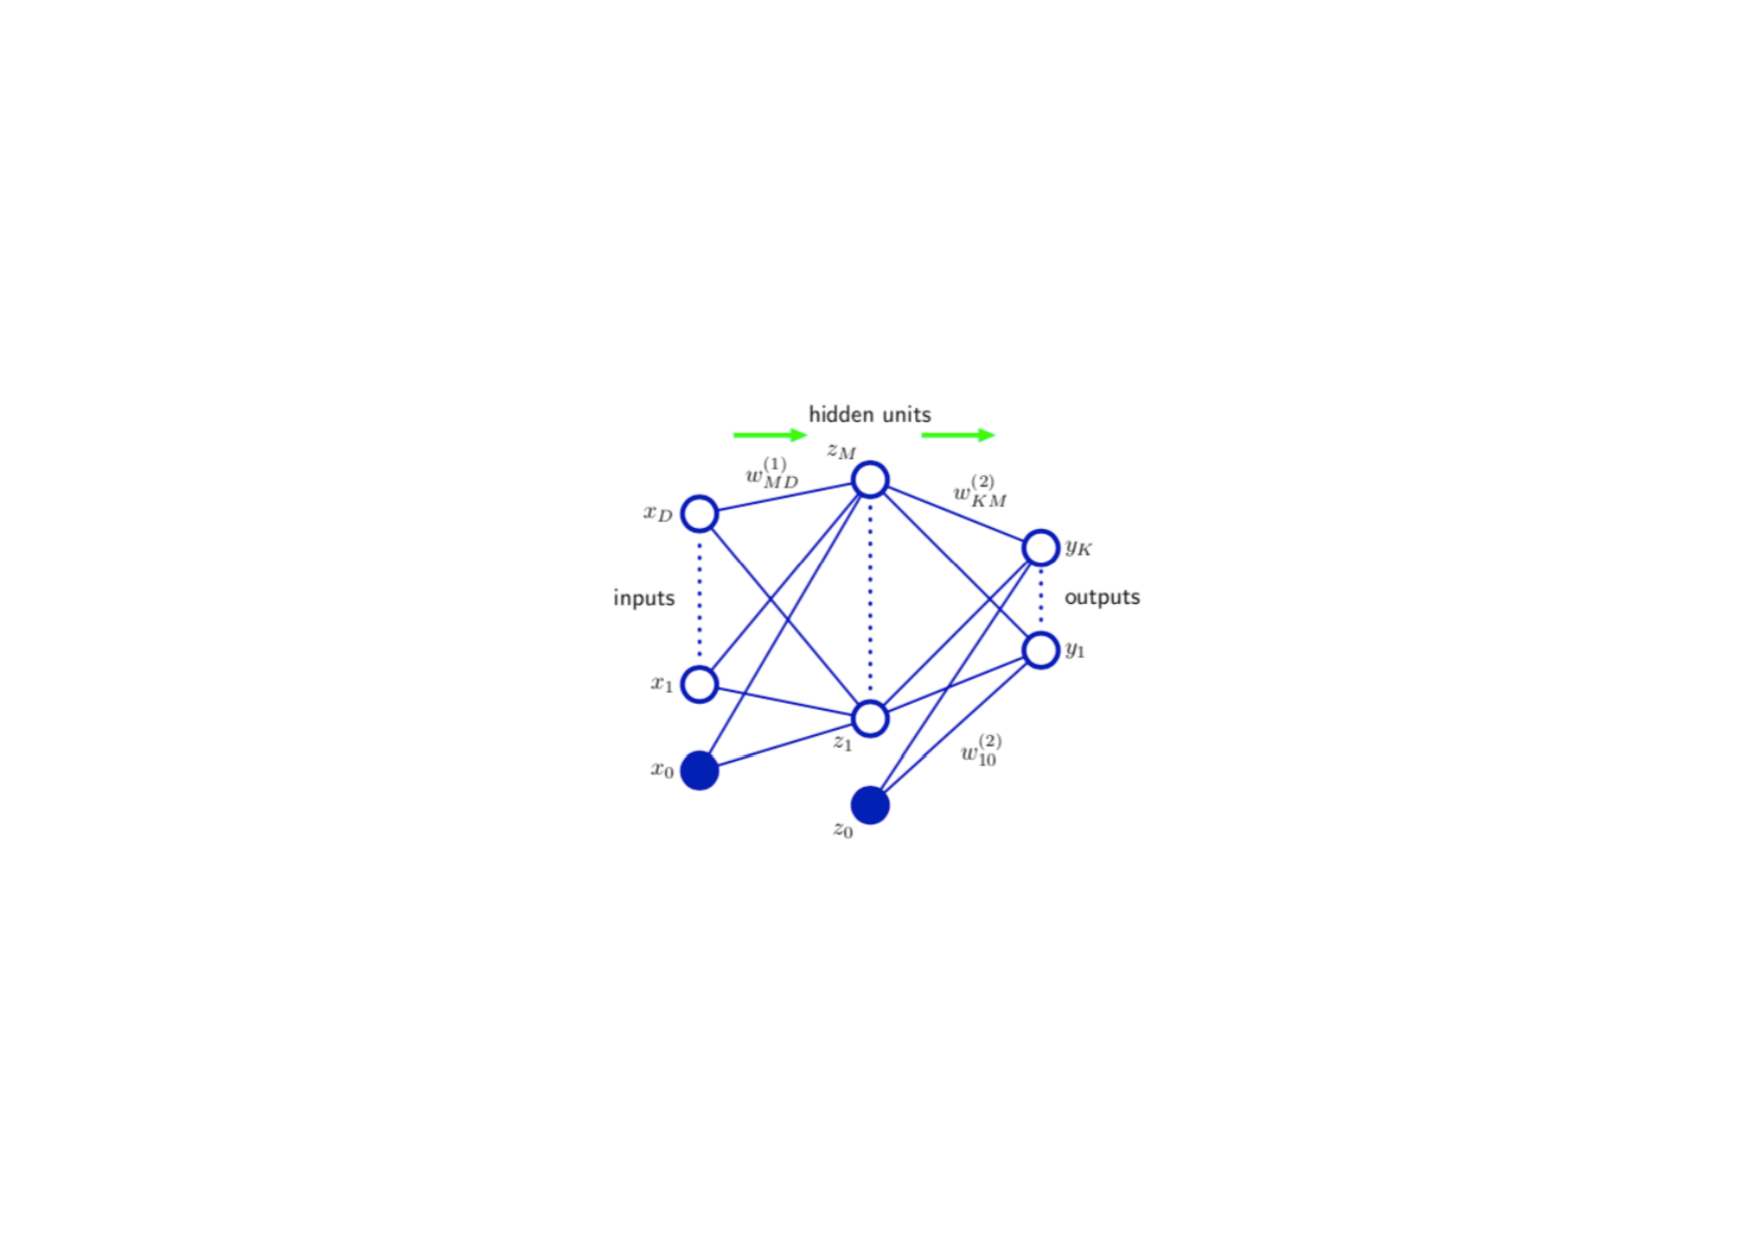
\includegraphics[width=0.6\textwidth]{figuras/RedeNeural.pdf}
     \caption{Arquitetura de uma rede neural \cite{Bishop}}
     \label{arqNN}
\end{figure}

Sinais fluem entre os neurônios através das arestas que estão associadas a um peso (w) que quantifica a sua importância. 
Nos neurônios é feito o processamento dos diversos sinais recebidos que, em seguida, aplica-se uma função, conhecida como função de ativação. 
Esta pode ser simplesmente uma combinação linear das entradas ponderadas pelos seus respectivos pesos, como pode ser função não linear como  sigmoid, 
tangente hiperbólica, entre outras \cite{Bishop}.   

\begin{figure}[H]
     \centering
     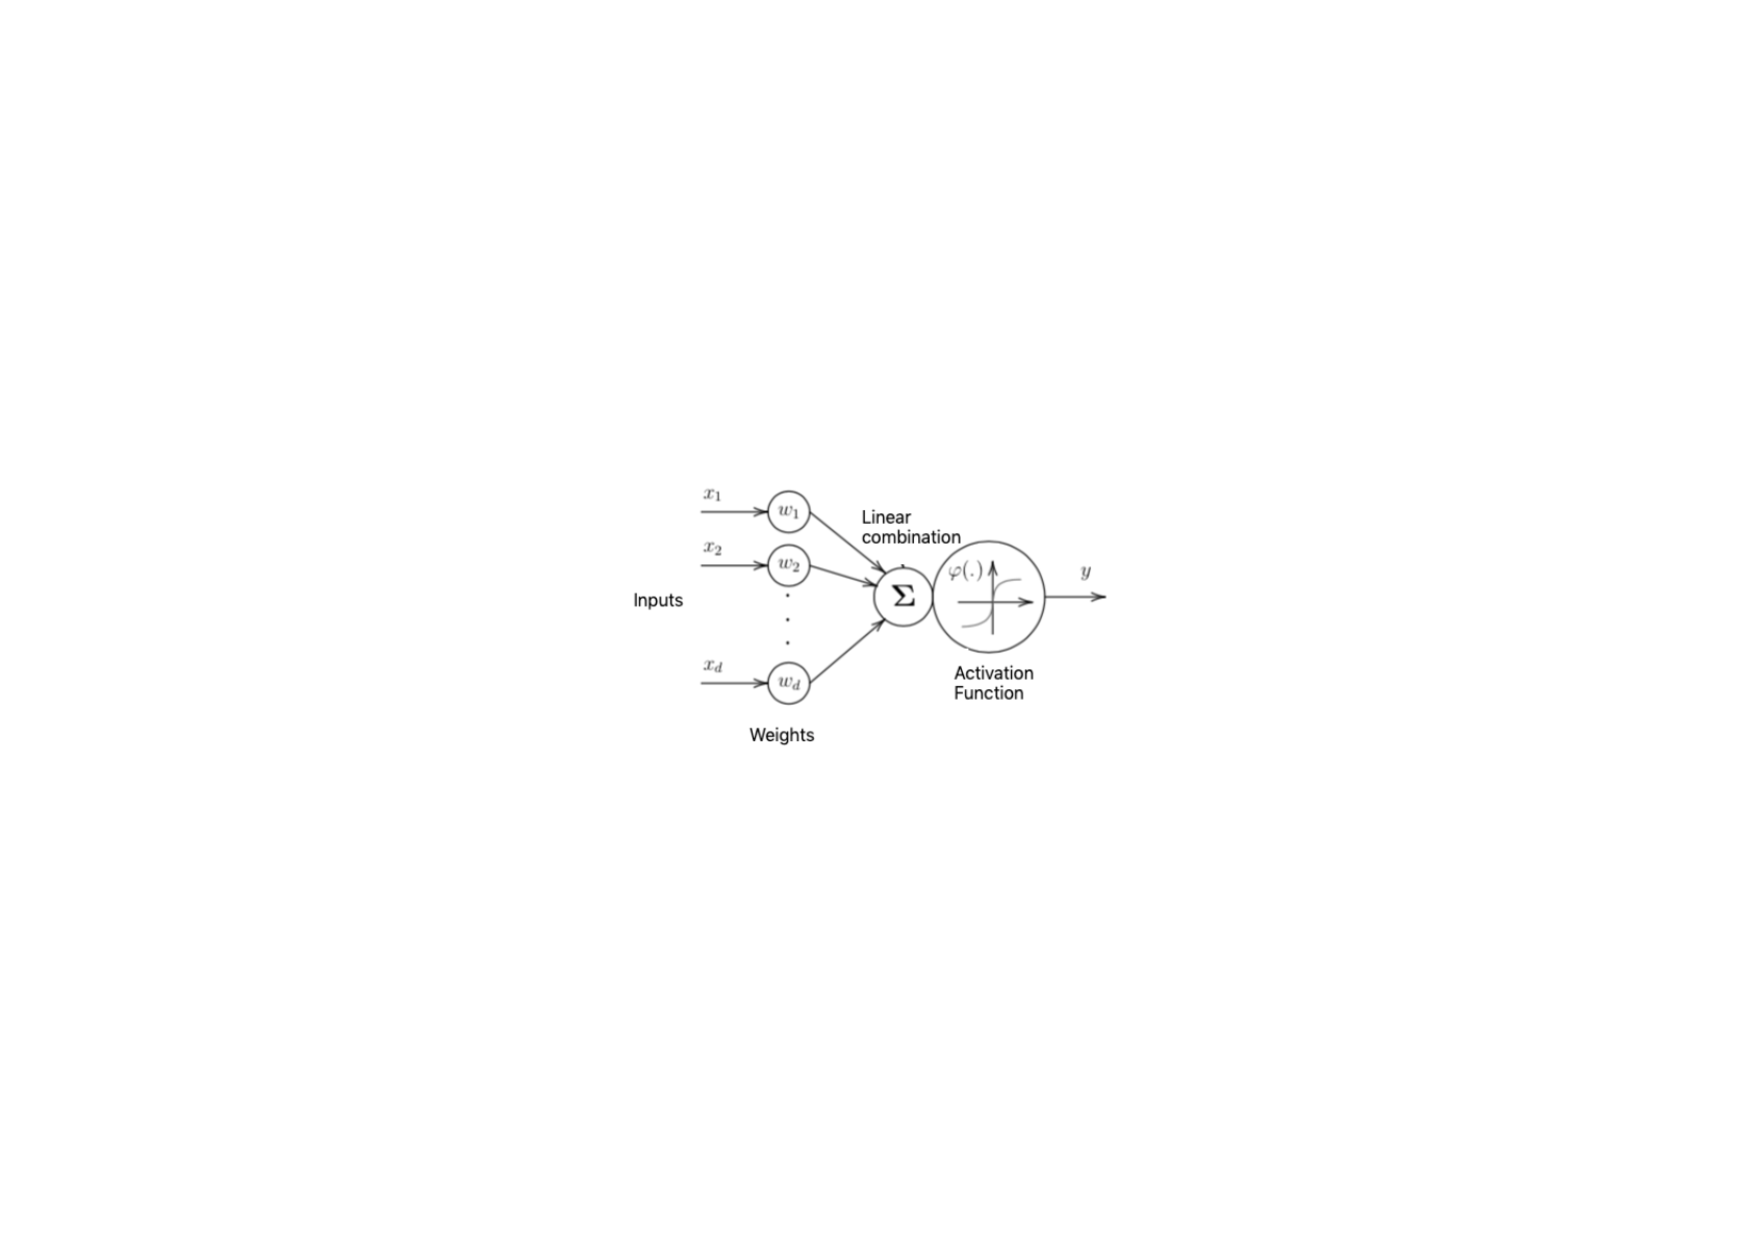
\includegraphics[width=0.6\textwidth]{figuras/ActivationFunc.pdf}
     \caption{Neurônio processando sinal \cite{Figueiredo}}
\end{figure}

Os pesos das arestas são ajustados durante a fase de treinamento,  de modo a orientar a rede a produzir a saída esperada para uma entrada específica. 
Nesta fase, é aplicado uma função de perda baseado na saída da rede. 
Existem diversas técnicas possíveis para minimizar a função de perda. 
Dentre elas, uma das mais tradicionais é a baseada no gradiente descendente, que atualiza os pesos conforme a equação a seguir. 

\begin{equation}
    w(t +1) = w(t) - n\nabla L(w(t)) 
\end{equation}

Onde w é o vetor de pesos, $n$ é uma constante positiva conhecida como taxa de aprendizagem, 
que quantifica o tamanho do ajuste dos parâmetros a cada iteração e $L$ é a função de perda. 
Um dos algoritmo mais utilizados para calcular o gradiente da função de perda e atualizar os parâmetros da rede é o \textit{Backpropagation} \cite{Bishop}. 

No contexto deste trabalho, as funções de perda estarão fortemente relacionadas ao valor de Retorno R e a função de Valor V apresentadas na seção anterior. 


\subsection{Método Actor-Critic}

O método Ator-Crítico (AC) é um procedimento que tem como objetivo otimizar a política de um MDP \cite{AC}. 
Ele é composto por dois componentes principais: o Ator e o Crítico. 
O Ator é aquele que seleciona as ações baseado nos estados, i.e, desempenha a função da política em um MDP. 
O Crítico, como o nome sugere, avalia a ação selecionada pelo Ator, estimando o vantagem de estar no estado alcançado. 
Assim, o Crítico é representado pela função de Valor do MDP. 
Tanto o Ator quanto o Crítico serão estimados por uma rede neural profunda cujos parâmetros serão ajustados utilizando a técnica \textit{Proximal Policy Optimization} \cite{PPO}.


\subsection{PPO}

A técnica \textit{Proximal Policy Optimization} é um modelo de aprendizado por reforço profundo que define funções de perda para ajustar os pesos das redes neurais pertencentes à arquitetura do método AC \cite{PPO}. 

Uma vez que o Crítico objetiva estimar o valor de V, o ajuste dos seus parâmetros ($W$) é feito através de um gradiente descendente a fim de minimizar o quadrado da diferença entre a saída da rede ($\hat{V}(W)$) e o V observado ($V^{obs}$) \cite{PPO}:


\begin{equation}
    L^{VF}_t(W) = (\hat{V}_t(W) - {V_t}^{obs})^2 
\end{equation}

\noindent
Uma dos principais motivações do PPO é, durante o processo de otimização do MDP, evitar atualizações de política muito grandes. 
Para isto, \cite{PPO} força com que a razão entre a política atual e a política anterior ($r_t(\Theta)$) seja limitada a um intervalo conveniente. 

\begin{equation}
    r_t(\Theta) = \frac{\pi_\Theta}{\pi_{\Theta old}}
\end{equation}

\noindent
Desta forma, para ajustar os parâmetros ($\Theta$) do Ator, \cite{PPO} define a seguinte função objetivo a ser maximizada por um gradiente ascendente:

\begin{equation}
   L^{CLIP}(\Theta) = \hat{E}_t [min(r_t (\Theta) \hat{A}_t, clip(r_t (\Theta), 1-\epsilon, 1+\epsilon) \hat{A}_t)]
\end{equation}

\noindent
Onde $\epsilon$ é uma constante que o \cite{PPO} sugere ser igual a 0.2. $\hat{A}_t$ é definido como a estimativa da função de vantagem, que corresponde ao benefício de selecionar uma ação $a$ no estado $s$, em comparação com uma seleção aleatória de uma ação no estado s. Em outras palavras, é a diferença entre Q e V:

\begin{equation}
   A = Q(s,a) - V(s)
\end{equation}

A função objetivo $L^{CLIP}(\Theta)$ é a esperança do mínimo de dois termos: $r_t(\Theta) \hat{A}_t$ e $clip(r_t (\Theta), 1-\epsilon, 1+\epsilon) \hat{A}_t$. O primeiro direciona a política a selecionar ações que maximizam a função de vantagem. O segundo é uma versão truncada do primeiro, onde é aplicado um \textit{clip} no $r_t(\Theta)$ de modo a garantir que a nova política não se distancie muito da política anterior. 

Uma vez que o aprendizado das redes do AC são dependentes entre si, \cite{PPO} sugere uma função objetivo única para treinar ambos:

\begin{equation}
   L_t ^{PPO} (\Theta) = \hat{E}_t[L_t ^{CLIP} (\Theta) - c_1 L_t ^{VF} (\Theta) + c_2 S(s_t)]
\end{equation}

Onde $c_1$ e $c_2$ são constantes e $S$ é definido por \cite{PPO} como um bônus de entropia que garante que o agente explore suficientemente o ambiente durante o treinamento.

\subsection{MDS}
\label{subsection:MDS}
Dado um conjunto de $n$ objetos e uma matriz $D = (dij)$ contendo a distância entre cada par $(i,j)$ de objetos, o objetivo do \textit{Metric Multidimensional Scaling} (MDS) é encontrar, 
para um objeto qualquer $Xi$, uma representação vetorial $Xi = [xi1,...,xim]$ tal que $||Xi - Xj|| = dij$.
Para isto, o método busca minimizar a diferença entre $||Xi - Xj||$ e $dij$ através da seguinte função de perda, conhecida por $Stress$:

\begin{equation}
    Stress(X1, X2, ..., Xn) = \sqrt{\sum_{i \neq j = 1}^{n} (d_{ij} - ||X_i - X_j||)^2}
 \end{equation}

{\color{red} Explicar como essa função é minimizada. Daria pra fazer pelo Gradient descendente mas aparentemente o mais usado é o SMACOF}

Neste trabalho utilizamos o MDS para codificar cada aminoácido em uma representação vetorial
que respeita a matriz de distâncias pré definidas por \cite{aminodist}. 

{\color{red} Sklearn cita Nonmetric multidimensional scaling: a numerical method” Kruskal, J. Psychometrika, 29 (1964)}














